\documentclass[a4paper]{article}

\usepackage{url}
\usepackage{amsmath}
\usepackage{verbatim}   		% Useful for program listings
\usepackage[T1]{fontenc}        % For Swedish characters
\usepackage[utf8]{inputenc}
\usepackage{fancyvrb}           % For lists with tabulators
\fvset{tabsize=4}               % Tabulator size
\fvset{fontsize=\small}         % List font size
\usepackage{graphicx}			% Imports the graphicx package, useful for images
% \usepackage{}

\title{Dragonfly Quadrotor UAV \\ Flight Control Board}
\author{Daniel Stenberg \\ Adam Steineck}

\date{May, 2015}         		% Today's date if not specified



\begin{document}                % Start of document

\maketitle                      % Prints the title defined above with
                                % \title, \author and \date

\begin{center}   
\vspace{64pt}                  

\includegraphics[scale=1.6]{images/AF_Logotype20141_Black.png}
\vspace{16pt}
\\ \large ÅF Embedded Systems
\end{center}

\newpage

\tableofcontents	% Insert table of contents

\newpage

\section{Introduction}

The \emph{Dragonfly} project is an internal competence enhancement project for ÅF employees. The goal is to combine technology, competence and experience from various engineering fields in order to construct a highly advanced quadrotor UAV system. The focus of the Flight Control Board development deals with low-level maneuvering of the aircraft, calculating motor command based on a feedback control system. Some of the major technologies deployed to attain this are control theory, electronics and software development.

\section{System description}

	\subsection{Flight dynamics}
	
	\subsection{Motors}

\section{Control}

	\subsection{Controller design}
	
	\subsection{Attitude control}
	
	\subsection{Estimation theory}

Reference to sample Figure \ref{fig:sampleimage}.

\begin{figure}[h]
    \centering
    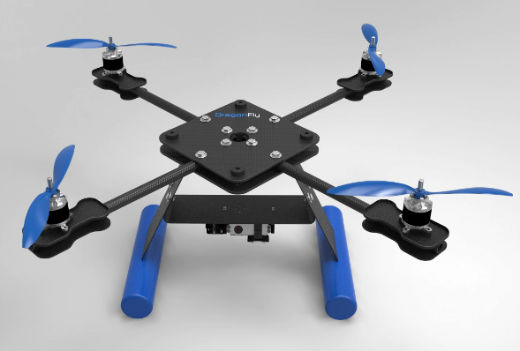
\includegraphics[scale=0.4]{images/quad_rendered.jpg}
    \caption{Sample image}
    \label{fig:sampleimage}
\end{figure}

Sample equation below in (\ref{eq7}).

\begin{equation}
\min e^{x_1} + x_{1}^2 + x_{1}x_{2} + \mu (\dfrac{1}{2}x_1 + x_2 - 1)^2
\label{eq7}
\end{equation}

Sample reference to \cite{stenberg}.

\section{Hardware}

\subsection{STM32F3Discovery}
The STM32F3Discovery is an evaluation board provided by STMicroelectronics. It features an STM32F303VCT6 microprocessor based on the ARM Cortex-M4 core. For evaluation purposes, the board has been fitted with accelerometer, magnetometer and gyroscope sensors, an on-board ST-Link/V2 debugger/programmer, various LED:s, extension headers for all I/O pins and more.

\begin{itemize}
  \item CPU speed: $72$ MHz
  \item ROM: 256 kB Flash
  \item SRAM: 48 kB (40 kB available to user)
  \item I/O pins: LQFP100 pin package with pins attached to extension header
  \item On-board ST-LINK/V2 programming and debugging device
  \item Power supply: From USB bus or from an external 3 V or 5 V supply voltage
  \item L3GD20 MEMS gyroscope
  \item LSM303DLHC MEMS accelerometer and magnetometer
  \item 10 LEDs
  \item Two pushbuttons (User and Reset)
  \item USB USER Mini-B connector
\end{itemize}

\section{Software}

\begin{thebibliography}{99}
\bibitem[1]{stenberg} Model-based Design Development and Control of a Wind Resistant Multirotor UAV, C. Månsson, D. Stenberg, Lunds Tekniska Högskola 2014
\end{thebibliography}

\end{document}                  % Slut p� dokumentet
